% Generated from main.typ. Typst is authoritative; regeneration overwrites this file.
\documentclass{qlnotes-export}

\title{MATH 597: Measure Theory}
\subtitle{Typst-first course notes and worked homeworks}
\author{Qiulin Fan}
\date{Winter 2025}

\begin{document}
\mainmatter
\chapter{Homework 2: on Carathéodory's and Hahn-Holmogrov Thm(40/40)}\label{homework-2-on-carathuxe9odorys-and-hahn-holmogrov-thm4040}

\emph{None of the following questions will be graded. Do them, but do not hand them in}.

\section{The Borel--Cantelli Lemma}\label{the-borelcantelli-lemma}

Let \((X,\mathcal{A},\mu)\) be a measure space. Let \(A_{i} \in \mathcal{A}\) for \(i \in {\mathbb{N}}\), and suppose that

\[\sum\limits_{i = 1}^{\infty}\mu(A_{i}) < \infty.\]

(a) Prove that \(\mu(\operatorname{lim\, sup}_{i}A_{i}) = 0\), where

\[\operatorname{lim\, sup}\limits_{i}A_{i} = \left\{ {x \in X \mid x \in A_{i}\ \text{for infinitely many}\ i} \right\}.\]

(By the way, why is \(\operatorname{lim\, sup}_{i}A_{i}\) measurable?)

(b) Conversely, is it true that if \(A_{i} \in \mathcal{A}\) for \(i \in {\mathbb{N}}\), and \(\mu(\operatorname{lim\, sup}_{i}A_{i}) = 0\), then \(\sum_{i}\mu(A_{i}) < \infty\)? Provide a proof or a counterexample. (Wrong)

\begin{qlremark}{Remark}

% qlnotes: kind=theorem; id=thm-hw02-on-carath-odorys-hahn-kolmogrov-thm-borel-cantelli-lemma; concepts=borel-cantelli-lemma; aliases=Borel–Cantelli Lemma
\begin{theorem}{Borel--Cantelli Lemma}\label{thm-hw02-on-carath-odorys-hahn-kolmogrov-thm-borel-cantelli-lemma}

一个 measure 和有限的 set seq, 其 \(\lim\sup\) (出现 infinitely many times 的元素) 是零测的.

\end{theorem}

其实这是 trivial 的, 因为如果出现 infinitely many times 的元素不是零测的, say \(\mu(\lim\sup_{i}A_{i}) := k > 0\), 那么有 infinitely many 个 \(A_{i}\) 的测度大于等于 \(k\), 那么 \(\sum_{i = 1}^{\infty}\mu(A_{i}) > k \times \infty\) 就一定不是有限的了.\\
其 application: 一个 prob space 中, a ctbl seq of 事件发生的概率的和如果收敛, 那么它们包含的任何事件发生无穷多次的概率为 0，意味着事件至多发生有限次 (almost surely).

\end{qlremark}

\section{The Completion of a Measure Space}\label{the-completion-of-a-measure-space}

Let \((X,\mathcal{A},\mu)\) be a measure space, and set

\[\bar{\mathcal{A}} := \left\{ {E \cup F \mid E \in \mathcal{A}\ \text{and}\ F\ \text{is a}\ \mu\ \text{-subnull set}} \right\}.\]

(a) Prove that \(\bar{\mathcal{A}}\) is a \(\sigma\)-algebra. (b) Define \(\bar{\mu}(A) := \mu(E)\) if \(A = E \cup F \in \bar{\mathcal{A}}\). Prove that \(\bar{\mu}\) is a well-defined measure on \(\bar{\mathcal{A}}\). (c) Prove that \(\bar{\mu}\) extends \(\mu\) (i.e., \(\bar{\mu}(A) = \mu(A)\) if \(A \in \mathcal{A}\)). (d) Prove that \textbf{\(\bar{\mu}\) is the unique extension of \(\mu\) to \((X,\bar{\mathcal{A}})\)}. In other words, prove that if \(\mu'\) is another measure on \((X,\bar{\mathcal{A}})\) that extends \(\mu\), then \(\mu' = \bar{\mu}\). (e) Prove that \textbf{\(\bar{\mu}\) is complete}. (f) Suppose \((X,\mathcal{A}',\mu')\) is another complete measure space that extends \((X,\mathcal{A},\mu)\) (i.e., \(\mathcal{A} \subset \mathcal{A}'\) and \(\left. \mu' \middle| {}_{\mathcal{A}} = \mu \right.\)). Show that \textbf{\(\bar{\mathcal{A}} \subset \mathcal{A}'\) and \(\left. \mu' \middle| {}_{\bar{\mathcal{A}}} = \bar{\mu} \right.\).} \textbf{Hint:} Start by reading Theorem 1.9 in Folland.

\begin{proof}

略.(嘻嘻)

\end{proof}

\section{The Hahn--Kolmogorov Extension as a Completion}\label{the-hahnkolmogorov-extension-as-a-completion}

Let \((X,\mathcal{A}_{0},\mu_{0})\) be a \(\sigma\)-finite measure pre-measure space, and \((X,\mathcal{A},\mu)\) its Hahn--Kolmogorov extension. Prove that \((X,\mathcal{A},\mu)\) is the completion of its restriction to the \(\sigma\)-algebra \(\langle\mathcal{A}_{0}\rangle\) generated by \(\mathcal{A}_{0}\).

\begin{proof}

Proved in lec notes.

\end{proof}

\emph{Some of the following questions will be graded. Do them, and do hand them in}.

\section{\texorpdfstring{\(\mu(\varnothing) = 0\) 的定义并非 redundant}{\textbackslash mu(\textbackslash varnothing) = 0 的定义并非 redundant}}\label{muemptyset-0-ux7684ux5b9aux4e49ux5e76ux975e-redundant}

Let \((X,\mathcal{A})\) be a measurable space. Is the condition \(\mu(\varnothing) = 0\) in the definition of a measure on \((X,\mathcal{A})\) redundant? In other words, if \(\mu:\mathcal{A}\rightarrow\lbrack 0,\infty\rbrack\) is a function such that

\[\mu\left( {\bigcup\limits_{i = 1}^{\infty}A_{i}} \right) = \sum\limits_{i = 1}^{\infty}\mu(A_{i}),\]

for any disjoint subsets \(A_{i} \in \mathcal{A}\), \(i \in {\mathbb{N}}\), does it follow that \(\mu(\varnothing) = 0\)? If not, what can you say?

\begin{proof}

It does not follow.\\
Counterexample: Consider \(\mu(E) = \infty\forall E \in \mathcal{A}\).\\
This measure satisfies the countably disjoint additivity condition, since for every disjoint sequence of sets in \(\mathcal{A}\), \(\mu\left( {\bigcup_{i = 1}^{\infty}A_{i}} \right) = \sum_{i = 1}^{\infty}\mu(A_{i}) = \infty\) has infinite measure.

\end{proof}

\section{\texorpdfstring{measurable set seq 的 limit 也 measurable (且如果 seq tail \(\sigma\)-finite \(\Longrightarrow\) limit commute )}{measurable set seq 的 limit 也 measurable (且如果 seq tail \textbackslash sigma-finite \textbackslash Longrightarrow limit commute )}}\label{measurable-set-seq-ux7684-limit-ux4e5f-measurable-ux4e14ux5982ux679c-seq-tail-sigma-finite-implies-limit-commute}

Let \((X,\mathcal{A},\mu)\) be a measure space, and let \(A_{i} \in \mathcal{A},i \in {\mathbb{N}}\). Assume that the sets \(A_{i}\) converge to the set \(A \subset X\) in the sense that: - If \(x \in A\), then \(x \in A_{i}\) for all but finitely many \(i\); - If \(x \notin A\), then \(x \notin A_{i}\) for all but finitely many \(i\).

\textbf{(a) Prove that \(A\) is measurable, that is, \(A \in \mathcal{A}\).}

\begin{proof}

Deduing from the conditions: If \(x \in A\), then \(x \in A_{i}\) for all but finitely many \(i\); \(\Longrightarrow\) \(A \subset \operatorname{lim\, inf}A_{i}\) If \(x \notin A\), then \(x \notin A_{i}\) for all but finitely many \(i\). \(\Longrightarrow\) if \(x \in A_{i}\) for all but finitely many \(i\) then \(x \in A\) \(\Longrightarrow\) \(\operatorname{lim\, sup}A_{i} \subset A\) Thus

\[\operatorname{lim\, sup}A_{i} \subset A \subset \operatorname{lim\, inf}A_{i}\]

\textbf{}

Claim1: For any sequence of sets \((A_{i})_{i \in {\mathbb{N}}}\), we have

\[\operatorname{lim\, inf}A_{i} \subset \operatorname{lim\, sup}A_{i}\] Proof of Claim 1: Follows trivially from the definition, since \(x \notin A_{i}\) for all but finitely many \(i\) \(\Longrightarrow\) \(x \notin A_{i}\) for infinitely many \(i\).\\
\strut \\
Combining claim (1) with (2.1) we have

\[\operatorname{lim\, sup}A_{i} = A = \operatorname{lim\, inf}A_{i}\]

\textbf{Claim 2: For any sequence of sets \((A_{i})_{i \in {\mathbb{N}}}\) in a \(\sigma\)-algebra, \(\operatorname{lim\, inf}_{i}Ai\) and \(\operatorname{lim\, sup}_{i}A_{i}\) is also in the \(\sigma\)-algebra.}\\
Proof of Claim 2: This follows from the def and fact that union and intersection of a countable sequence sets in a \(\sigma\)-algebra is also in this \(\sigma\)-algebra. We have

\begin{center}

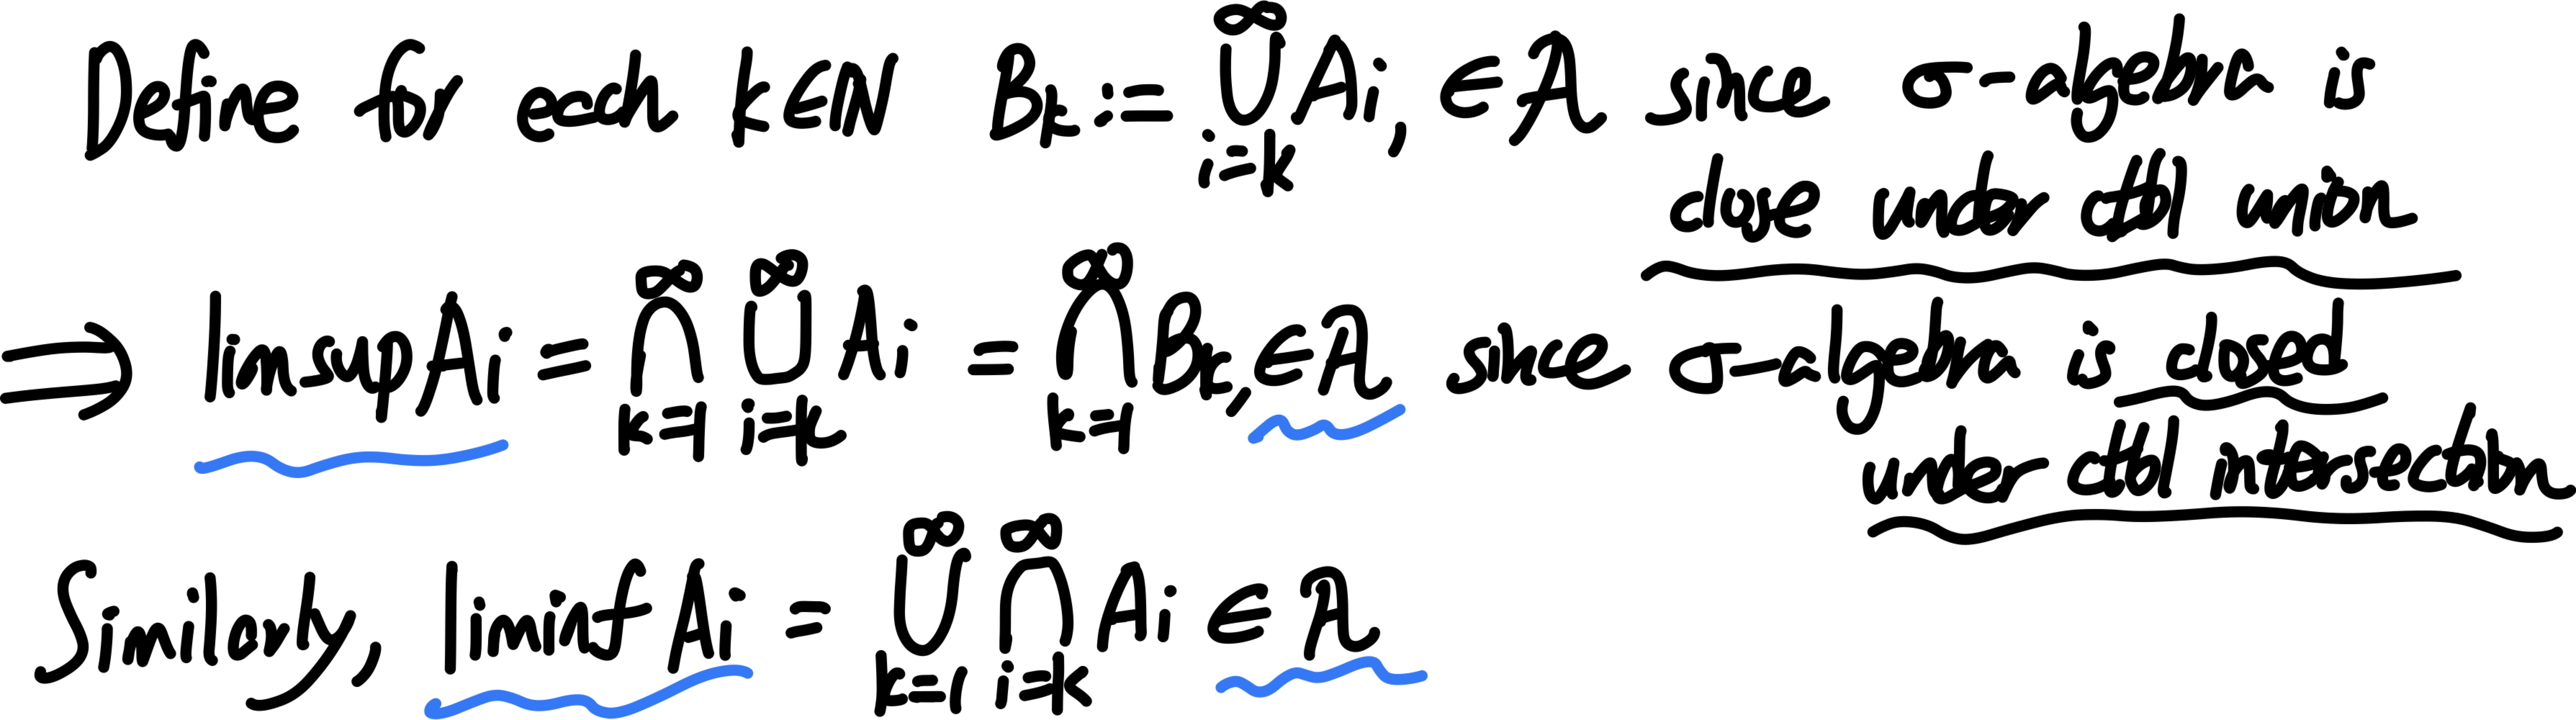
\includegraphics[width=0.8\linewidth,height=\textheight,keepaspectratio]{assets/main--figure-raster-003.jpg}

\end{center}

This finishes the proof of Claim 2.\\
Combining claim 2 with (2.2), \(A \in \mathcal{A}\), this finishes the proof.\\

\end{proof}

\textbf{(b) Prove that if there exists \(n \geq 1\) such that \(\mu\left( {\bigcup_{i = n}^{\infty}A_{i}} \right) < \infty\), then \(\mu(A) = \lim_{i}\mu(A_{i})\).}

\begin{proof}

\begin{center}

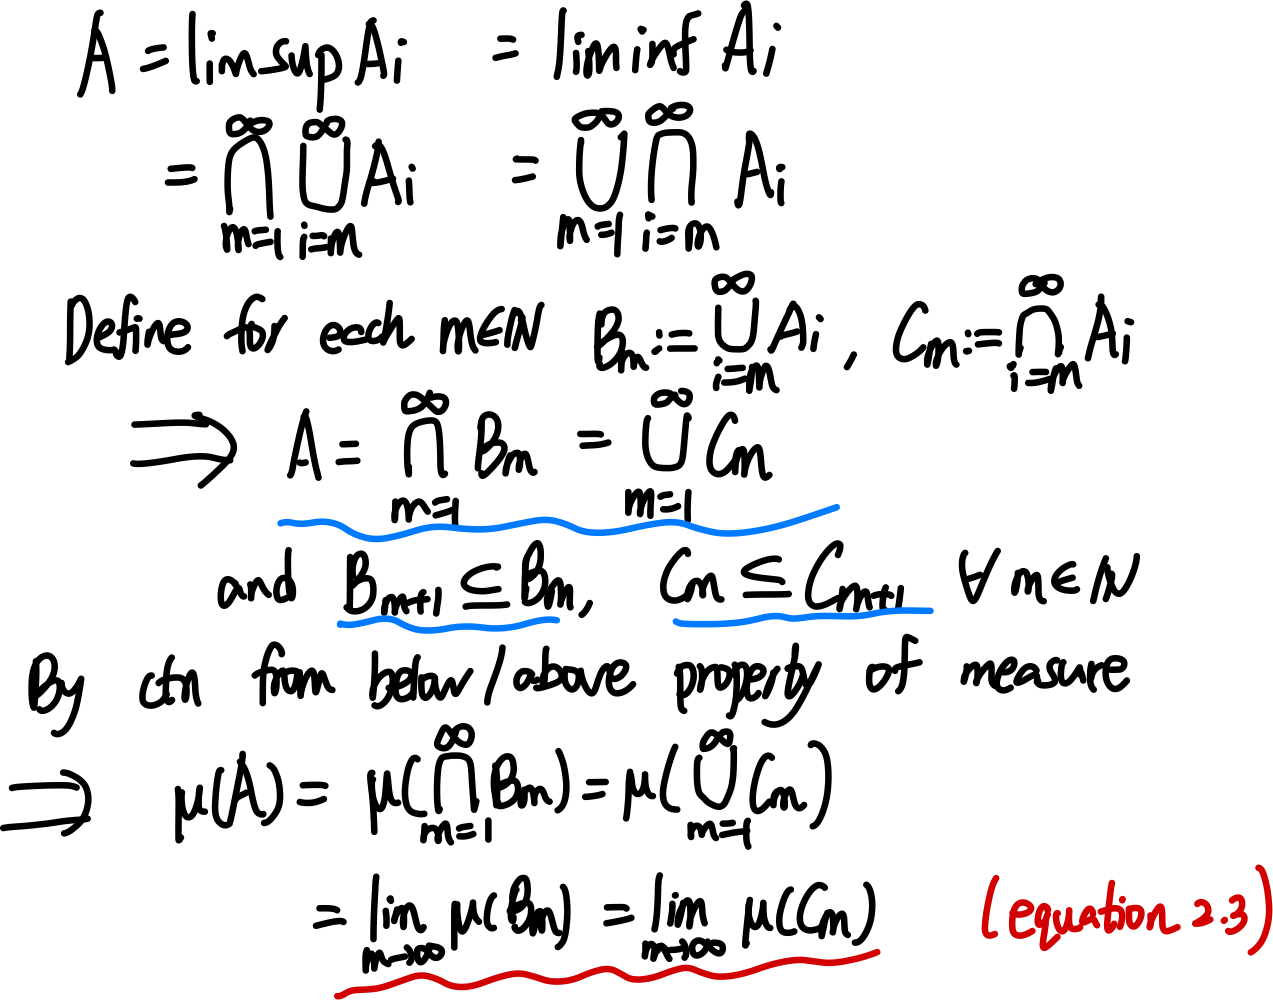
\includegraphics[width=0.7\linewidth,height=\textheight,keepaspectratio]{assets/main--figure-raster-004.png}

\end{center}

\begin{center}

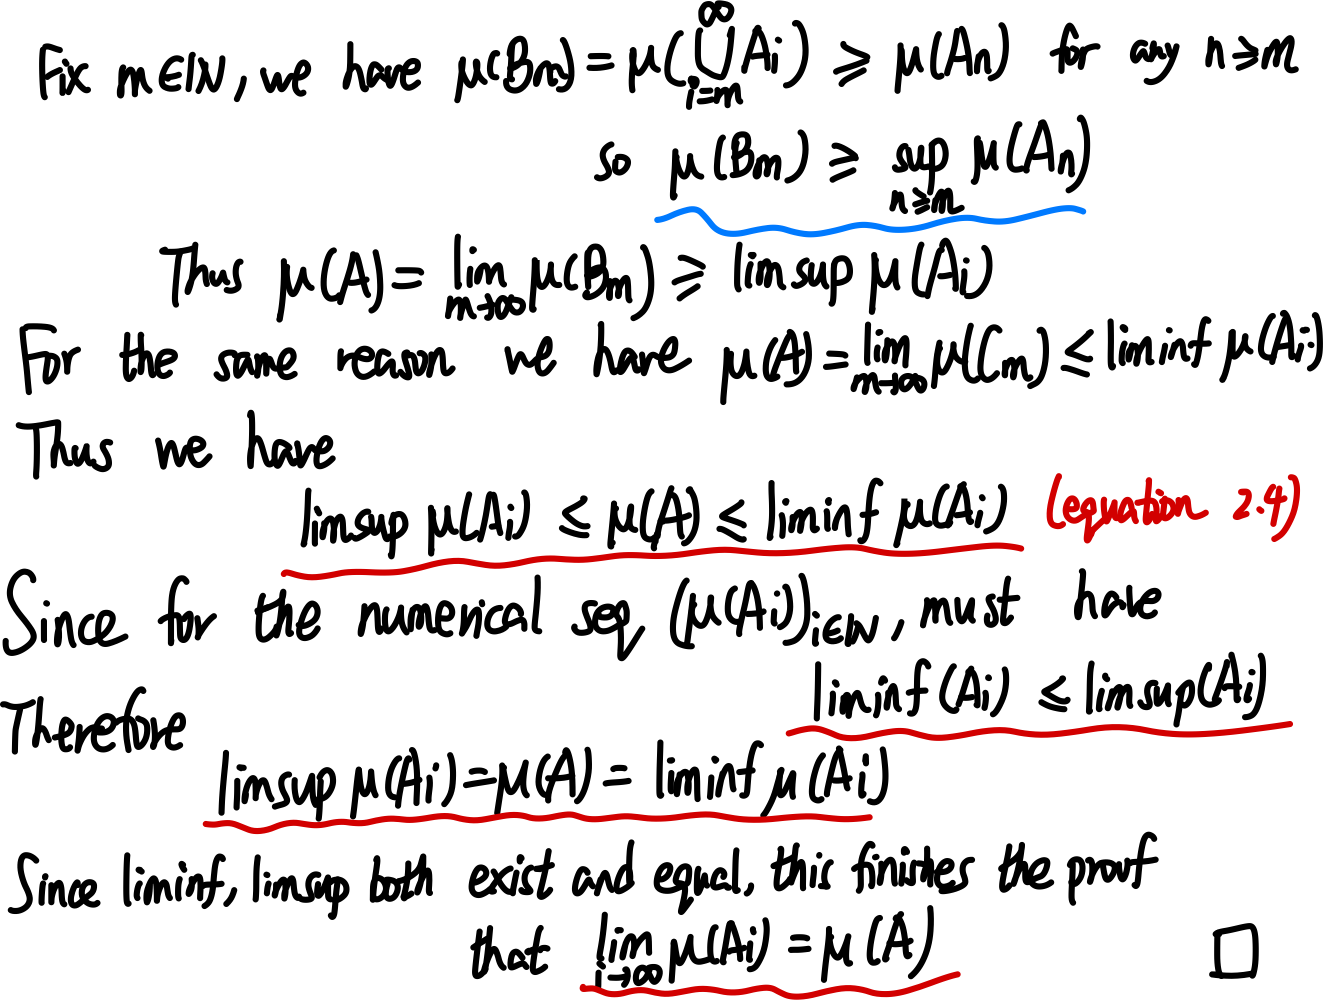
\includegraphics[width=0.7\linewidth,height=\textheight,keepaspectratio]{assets/main--figure-raster-005.png}

\end{center}

\end{proof}

\textbf{(c) Give an example showing that the condition in (b) is necessary}.

\begin{qlsolution}{Solution}

Let \(\mu\) be the Lebesgue measure defined on \(\mathcal{B}({\mathbb{R}})\). We set for each \(i \in {\mathbb{N}}\) that

\[A_{i} = (i,i + 1)\]

Since this is an interval, it is Lebesgue measurable. Note that no element of any \(A_{i}\) show up infinitely many times in the sequence. So

\[\operatorname{lim\, inf}A_{i} = \operatorname{lim\, sup}A_{i} = \varnothing\]

So \(A = \varnothing\), we have \(\lim_{i}\mu(A_{i}) = 0\). But we have \(\lim_{i}\mu(A_{i}) = 1\) since it is true for every \(i\).\\
In this case, \(\mu(\bigcup_{i = 1}^{\infty}A_{i}) = \infty\), which causes (b) to fail.

\end{qlsolution}

\textbf{Hint:} In analysis, it is often fruitful to use \(\operatorname{lim\, sup}\) and \(\operatorname{lim\, inf}\) to study limits.\\

\section{measure space of two elements}\label{measure-space-of-two-elements}

Let \(X\) be a set with two elements, for example, \(X = \left\{ {O,Q} \right\}\).\\
\textbf{(a) Find all \(\sigma\)-algebras on \(X\).}

\begin{qlsolution}{Solution}

\begin{enumerate}
\item
  trivial \(\sigma\)-algebra:

  \[\mathcal{A}_{1} := \left\{ {\varnothing, X} \right\}\]
\item
  power set:

  \[\mathcal{A}_{2} := \mathcal{P}(X) = \left\{ {\varnothing,\left\{ O \right\},\left\{ Q \right\}, X} \right\}\]
\end{enumerate}

These are the only \(\sigma\)-algebras on \(X\).\\
\strut \\

\end{qlsolution}

\textbf{(b) Let \(\mathcal{A}\) be a \(\sigma\)-algebra on \(X\), and \(\mu\) a measure on \((X,\mathcal{A})\). Is \(\mu\) necessarily complete? Provide a proof or a counterexample.}

\begin{qlsolution}{Solution}

It is not necessarily complete.\\
Cosider the trivial \(\sigma\)-algebra:\(\mathcal{A}_{1} := \left\{ {\varnothing, X} \right\}\), and set \(\mu\) as that \(\mu(\varnothing) = \mu(X) = 0\). This makes \(X\) a null set, so \(\left\{ O \right\},\left\{ Q \right\}\) are subnull sets, but they are not measurable by \(\mu\).\\
\strut \\

\end{qlsolution}

\textbf{(c) Find all outer measures \(\mu^{\ast}\) on \(X\). For each outer measure on \(X\), find the \(\sigma\)-algebra of \(\mu^{\ast}\)-measurable sets (see Carathéodory's theorem).}

\begin{qlsolution}{Solution}

Suppose \(\mu^{\ast}\) is an outer measure on \(X\). Since \(\mathcal{P}(X)\) only has four elements: \(\varnothing\), \(\left\{ O \right\}\), \(\left\{ Q \right\}\), \(X\); and the outer measure of \(\varnothing\) is 0, so we first parametrize \(\mu^{\ast}\) by:

\[a := \mu^{\ast}(\left\{ O \right\}),\quad b := \mu^{\ast}(\left\{ Q \right\}),\quad c := \mu^{\ast}(X).\]

\end{qlsolution}

Then \(\mu^{\ast}\) is well-defined iff it satisfies:

\begin{enumerate}
\item
  \(a,b \leq c\)
\item
  \(c = \mu^{\ast}(\left\{ O \right\} \cup \left\{ Q \right\}) \leq \mu^{\ast}(\left\{ O \right\}) + \mu^{\ast}(\left\{ Q \right\}) = a + b.\)
\end{enumerate}

Any \((a,b,c) \in \lbrack 0,\infty\rbrack^{3}\) satisfying

\[\max(a,b) \leq c \leq a + b,\]

can make \(\mu^{\ast}\) a well-defined outer measure on \(X\).\\
Therefore

\[S := \left\{ {\text{all}\ \sigma\ \text{-algebra on}\ X} \right\} = \left\{ {\mu^{\ast}:\mathcal{P}(X)\rightarrow\lbrack 0,\infty\rbrack \mid \max(\mu^{\ast}(\left\{ O \right\}),\mu^{\ast}(\left\{ Q \right\})) \leq \mu^{\ast}(X) \leq \mu^{\ast}(\left\{ O \right\}) + \mu^{\ast}(\left\{ Q \right\})} \right\}\]

\hfill\break
Now we specify the \(\sigma\)-algebra of \(\mu^{\ast}\)-measurable sets for each \(\mu^{\ast} \in S\).\\
By Carathéodory's criterion, a set \(E \subset X\) is \(\mu^{\ast}\)-measurable iff for all \(A \subset X\),

\[\mu^{\ast}(A) = \mu^{\ast}(A \cap E) + \mu^{\ast}(A \cap E^{c}).\]

Note that \(\varnothing\), \(X\) are always measurable since for any \(A \subset X\), \(A \cap \varnothing = \varnothing, A \cap (\varnothing)^{c} = A\); and \(A \cap X = A, A \cap (X)^{c} = \varnothing\). So it suffices to check for \(\left\{ O \right\},\left\{ Q \right\}\). We first check for \(\left\{ O \right\}\). \(\left\{ O \right\}\) is \(\mu^{\ast}\)-measurable iff \(\mu^{\ast}(A) = \mu^{\ast}(A \cap \left\{ O \right\}) + \mu^{\ast}(A \cap \left\{ O \right\}^{c})\) for any choice of \(A\). There are only four possibilities for \(A\): \(\varnothing\), \(\left\{ O \right\}\), \(\left\{ Q \right\}\), \(X\).

\begin{enumerate}
\item
  If \(A = \varnothing\), both sides are 0, always stands.
\item
  If \(A = \left\{ O \right\}\), then \(\mu^{\ast}(\left\{ O \right\}) + \mu^{\ast}(\varnothing) = a + 0 = a\), always stands.
\item
  If \(A = \left\{ Q \right\}\), then \(\mu^{\ast}(\varnothing) + \mu^{\ast}(\left\{ Q \right\}) = 0 + b = b\), always stands.
\item
  If \(A = X\), then \(\mu^{\ast}(X) = c = \mu^{\ast}(\left\{ O \right\}) + \mu^{\ast}(\left\{ Q \right\}) = a + b\).
\end{enumerate}

Therefore \(\left\{ O \right\}\) is \(\mu^{\ast}\)-measurable iff \(c = a + b\). For the same reasoning, \(\left\{ Q \right\}\) is \(\mu^{\ast}\)-measurable iff \(c = a + b\).\\
Thus we can conclude that:

\begin{enumerate}
\item
  If \(c = a + b\), \(\left\{ {\mu^{\ast}\ \text{-measurable sets}} \right\} = \mathcal{P}(X)\).
\item
  otherwise, \(\left\{ {\mu^{\ast}\ \text{-measurable sets}} \right\} = \left\{ {\varnothing,X} \right\}\).
\end{enumerate}

\textbf{(d) Find an example of a collection \(\mathcal{E}\) of subsets of \(X\) with \(\varnothing,X \in \mathcal{E}\) and a function \(\rho:\mathcal{E}\rightarrow\lbrack 0,\infty\rbrack\) with \(\rho(\varnothing) = 0\) such that \(\mathcal{E} \not\subset \mathcal{A}\), where \(\mathcal{A}\) is the Carathéodory \(\sigma\)-algebra for the outer measure \(\mu^{\ast}\) induced by \((\mathcal{E},\rho)\).}

\begin{qlsolution}{Solution}

Consider \(\mathcal{E} = \left\{ {\varnothing,X,\left\{ O \right\}} \right\}\), with \(\rho\) such that \(\rho(\varnothing) = 0\), \(\rho(X) = 1\), \(\rho(\left\{ O \right\}) = 1\).\\
The outer measure \(\mu^{\ast}\) induced by \(\mu^{\ast}\) is: \(\mu^{\ast}(X) = 1\), \(\mu^{\ast}(\left\{ O \right\}) = 1\), \(\mu^{\ast}(\left\{ Q \right\}) = 1\). (the inf of length sum of sets covering \(\left\{ Q \right\}\) is 1, by taking \(\left\{ X \right\}\) as the covering.)\\
Since \(c \neq a + b\), by (4), the Carathéodory \(\sigma\)-algebra by \(\mu^{\ast}\) by \(\mathcal{E}\) is \(\left\{ {\varnothing,X} \right\}\), so \(\mathcal{E} \not\subset \mathcal{A}\).\\
\strut \\

\end{qlsolution}

\textbf{Remark:} The Hahn--Kolmogorov theorem states that if \(\mathcal{E} = \mathcal{A}_{0}\) is an algebra and \(\rho = \mu_{0}\) is a pre-measure, then \(\mathcal{A}_{0} \subset \mathcal{A}\). This exercise provides a counterexample when \(\mathcal{E}\) and \(\rho\) are general. 、

\section{\texorpdfstring{Hahn--Kolmogorov Collapse (when \(\mu_{0}\) not \(\sigma\)-finite)}{Hahn--Kolmogorov Collapse (when \textbackslash mu\_\{0\} not \textbackslash sigma-finite)}}\label{hahnkolmogorov-collapse-when-mu_0-not-sigma-finite}

Let \(X \subset {\mathbb{R}}\) be the set of dyadic rational numbers, that is, the set of numbers of the form \(\frac{r}{2^{n}}\), where \(r\) and \(n\) are integers. Let \(\mathcal{A}_{0} \subset \mathcal{P}(X)\) be the collection of finite unions of intervals of the form \((a,b\rbrack \cap X\), where \(- \infty \leq a < b \leq \infty\).

\textbf{(a) Prove that \(\mathcal{A}_{0}\) is an algebra.}

\begin{proof}

\begin{enumerate}
\item
  \(\varnothing \in \mathcal{A}_{0}\), since it is the empty union of intervals of the given form.
\item
  \textbf{Closed under complements}: Let \(A \in \mathcal{A}_{0}\). Then \(A\) is a finite union of intervals of the form \((a_{i},b_{i}\rbrack \cap X\). So

  \[\begin{matrix}
  {A^{c} \cap X} & {= X\backslash A} \\
   & {= X\backslash\bigcup\limits_{i = 1}^{n}((a_{i},b_{i}\rbrack \cap X))} \\
   & {= X \cap (\bigcap\limits_{i = 1}^{n}((a_{i},b_{i}\rbrack \cap X)^{c})} \\
   & {= X \cap (\bigcap\limits_{i = 1}^{n}(( - \infty,a_{i}\rbrack \cup (b_{i},\infty\rbrack))}
  \end{matrix}\]

  Note that finite intersection of intervals of the form \(( - \infty,a_{i}\rbrack\), \((b_{i},\infty\rbrack\) is still of this form. Hence \(A^{c} \cap X \in \mathcal{A}_{0}\).
\item
  \textbf{Closed under finite unions}: Suppose \(A_{1}\) and \(A_{2}\) are finite unions of intervals \(((a_{i},b_{i}\rbrack \cap X)\), then \(A_{1} \cup A_{2}\) is still a finite union of intervals of that form. (They either merge into one such interval, so are disjoint.) Hence \(A_{1} \cup A_{2} \in \mathcal{A}_{0}\). The same reasoning extends to any finite union.
\end{enumerate}

\textbf{This finishes the proof that \(\mathcal{A}_{0}\) is an algebra on \(X\).}\\
\strut \\

\end{proof}

\textbf{(b) Prove that the \(\sigma\)-algebra on \(X\) generated by \(\mathcal{A}_{0}\) equals \(\mathcal{P}(X)\).}

\begin{proof}

Since \(< \mathcal{A}_{0} > \subset \mathcal{P}(X)\), it suffices to show that \(\mathcal{P}(X) \subset < \mathcal{A}_{0} >\). Note that \(X\) is countable, so any set in \(\mathcal{P}(X)\) is a countable union of singleton sets. Thus it suffices to show that any singleton set \(\left\{ x \right\}\) where \(x \in X\) is in \(< \mathcal{A}_{0} >\), since if so, then any countable union of singleton sets from \(\mathcal{P}(X)\) is also in \(< \mathcal{A}_{0} >\), with implies that \(\mathcal{P}(X) \subset < \mathcal{A}_{0} >\)\\
Let \(x \in X\). Then we have:

\[\left\{ x \right\} = \bigcap\limits_{n = 1}^{\infty}((x - \frac{1}{2^{n}},\, x\rbrack \cap X),\]

since \(x\) is in the RHS set, and for any \(y < x\), we can find a \(n \in \mathcal{B}\) such that \(x - \frac{1}{2^{n}} > y\).\\
This finishes the proof that \(< \mathcal{A}_{0} > = \mathcal{P}(X)\).

\end{proof}

\textbf{(c) Define \(\mu_{0}:\mathcal{A}_{0}\rightarrow\lbrack 0,\infty\rbrack\) by \(\mu_{0}(\varnothing) = 0\) and \(\mu_{0}(A) = \infty\) for \(A \neq \varnothing\). Prove that \(\mu_{0}\) is a pre-measure on \(\mathcal{A}_{0}\)}

\begin{proof}

It suffices to show the countable disjoint additivity.\\
Let \((A_{i})_{i \in \mathcal{N}}\) be a sequence of disjoint sets in \(\mathcal{A}_{0}\).\\
Case 1: all \(A_{i} = \varnothing\), then \(\sqcup_{i \in \mathcal{N}}A_{i} = \varnothing\), so \(\mu_{0}( \sqcup_{i \in \mathcal{N}}A_{i}) = \sum_{i \in \mathcal{N}}\mu_{0}(A_{i}) = 0\).\\
Case 2: \(A_{k} \neq \varnothing\) for some \(k\), then \(\mu_{0}(A_{k}) = \infty\) and \(\sqcup_{i \in \mathcal{N}}A_{i} \neq \varnothing\). Thus \(\sum_{i \in \mathcal{N}}\mu_{0}(A_{i}) \geq \mu_{0}(A_{k}) = \infty = \mu_{0}( \sqcup_{i \in \mathcal{N}}A_{i})\).\\
The two cases cover all circumstances, finishing the proof.\\

\end{proof}

\textbf{(d) Prove that there exist infinitely many different measures \(\mu\) on \(\mathcal{P}(X)\) whose restriction to \(\mathcal{A}_{0}\) equals \(\mu_{0}\).}

\begin{proof}

Given \(n \in {\mathbb{N}}\), We define the "n-timed counting measure" on a \(\sigma\)-algebra \(S\) as:

\[\begin{matrix}
{\mu_{count_{n}}(E) := \{ n \times \#(E),\text{if}\ E\ \text{is finite}} \\
{\infty,\text{if}\ E\ \text{is infinite}}
\end{matrix}\]

\textbf{Claim 1: For any set \(X\) and any \(\sigma\)-algebra \(S\) on \(X\), the "n-timed counting measure" is a well-defined measure on \(S\), for all \(n \in {\mathbb{N}}\).}\\
Proof of claim 1: \(\mu_{count_{n}}(\varnothing) = 0\) since \(\text{card}(\varnothing) = 0\), and countable disjoint additivity trivially follows from the rule of counting.\\
\textbf{Claim 2: for any \(n \in {\mathbb{N}}\), \(\mu_{count_{n}}(E)\) on \(\mathcal{P}(X)\) restricted to \(\mathcal{A}_{0}\) equals \(\mu_{0}\).} Proof of claim 2: Let \(E \in \mathcal{A}_{0}\backslash\varnothing\), then \(E\) contains at least one interval of the form \((a,b\rbrack \cap X\), where \(- \infty \leq a < b \leq \infty\). Sicne \(a < b\), there are infinitely many elements in \((a,b\rbrack \cap X\), so \(\mu_{count_{n}}(E) = \infty\).\\
This finishes the proof of the original statement.\\

\end{proof}

\textbf{(e) Explain why (d) does not contradict the uniqueness part of the Hahn--Kolmogorov theorem (see Theorem 1.14 in Folland).}\\

\begin{qlsolution}{Solution}

This is because Hahn--Kolmogorov theorem requires \(\mu_{0}\) to be \(\sigma\)-finite to extend uniquely on \(< \mathcal{A}_{0} >\). But \(\mu_{0}\) here is not \(\sigma\)-finite.\\

\end{qlsolution}

\section{Nur für Verrückte (Only for nuts)}\label{nur-fuxfcr-verruxfcckte-only-for-nuts}

(It's really not necessary to attempt these problems. Do not, under any circumstances, hand them in!)

1. Let \((X,\mathcal{A},\mu)\) and \((Y,\mathcal{B},\nu)\) be measure spaces. Define a morphism from \((X,\mathcal{A},\mu)\) to \((Y,\mathcal{B},\nu)\) to be a map \(f:X\rightarrow Y\) that is measurable, that is, \(f^{- 1}(B) \in \mathcal{A}\) for all \(B \in \mathcal{B}\), and moreover measure preserving, in the sense that \(\mu(f^{- 1}(B)) = \nu(B)\) for all \(B \in \mathcal{B}\).

(a) Prove that measure spaces with measure-preserving maps as morphisms form a category. Denote this category by \(C_{3}\).

(b) Denote by \(C_{1}\) the category of sets, and by \(C_{2}\) the category of measurable spaces (see HW1). Consider the evident forgetful functors \(C_{3}\rightarrow C_{2}\) and \(C_{2}\rightarrow C_{1}\). Are these functors faithful? Are they full? Are they essentially surjective?
\end{document}
